\documentclass[]{article}
\usepackage[german]{babel}
\usepackage{graphicx}
\usepackage{tabularx}
\usepackage[backend=bibtex, natbib=true]{biblatex}
\usepackage{listings}
\usepackage{tikz}

\lstset{%
	basicstyle=\ttfamily\scriptsize,        % Code font, Examples: \footnotesize, \ttfamily
	keywordstyle=\color{blue!80!black},     % Keywords font ('*' = uppercase)
	commentstyle=\color{gray},              % Comments font
	numbers=left,                           % Line nums position
	numberstyle=\tiny,                      % Line-numbers fonts
	stepnumber=1,                           % Step between two line-numbers
	numbersep=5pt,                          % How far are line-numbers from code
	backgroundcolor=\color{gray!10!white},  % Choose background color
	frame=none,                             % A frame around the code
	tabsize=2,                              % Default tab size
	captionpos=b,                           % Caption-position = bottom
	breaklines=true,                        % Automatic line breaking?
	breakatwhitespace=false,                % Automatic breaks only at whitespace?
	showspaces=false,                       % Dont make spaces visible
	showstringspaces=false                  %
	showtabs=false,                         % Dont make tabls visible
	columns=flexible,                       % Column format
	morekeywords={},                        % Specific keywords
	stringstyle=\color{green!50!black},%
}%

\bibliography{bibliography}
%opening
%Here you can enter your names and titleof your report
\title{Dokumentation - Luftqualität in Innenräumen - Gruppe 1}
\author{Friedrich Just 1326699 \\ Stipe Knez 1269206 \\ Lucas Merkert 1326709 \\ Achim Glaesmann 1309221 \\ Max-Rene Konieczka 1211092 \\ Can Cihan Nazlier 1179244}

\begin{document}

	\begin{titlepage}
		\maketitle
		\thispagestyle{empty}
	\end{titlepage}
	\tableofcontents
	\setcounter{page}{1}
	\newpage
	
	
	\section{Projektthema}
	Die durch Covid-19 verursachte Pandemie prägte die letzten 2 Jahre der gesamten Welt. Insgesamt forderte die Krankheit etwa 5,18 Millionen Menschenleben. Dennoch ist das Thema aktueller denn je. Europaweit steigen die Infektionszahlen auf nie dagewesene Werte, während die im Sommer verabreichten Impfungen langsam an Effektivität verlieren. Ein Hauptrisiko zur Infektion besteht dabei in Innenräumen. Unser Auftrag besteht nun darin, ein System zu entwickeln welches in der Lage ist, das Infektionsrisiko einzelner Räume eines Gebäudes einzuschätzen und so einen Richtwert für den Anwender darstellt, wie er sein Verhalten diesem Wert anpassen kann. Realisiert werden soll dieses System über die Verwendung verschiedener Sensoren zur Erfassung mit dem Infektionsrisiko direkt verknüpfter physikalischer Größen. Die zur Ansteckung, vermutlich, wichtigen Aerosole, können dabei nur bedingt durch Masken zurückgehalten werden, es macht also Sinn abzuschätzen inwieweit die Luft eines Raumes durch Aerosole belastet ist. Da die direkte Messung von Aerosolen zeitaufwendig und schwer umsetzbar ist, konzentrieren wir uns hierbei auf Werte, die einen direkten Rückschluss auf die Ausatemmenge der Personen im Raum ermöglichen, mit der Annahme, dass die Aerosolkonzentration dabei direkt abhängig zur Ausatemmenge ist.\newline
	Um dies zu erreichen, bedienen wir uns folgender Sensoren: Dem CCS811 von Adafruit, dem SCD41 und dem SHT21 von Sensirion. Der CCS881 ist ein energieeffizienter digitaler Gassensor, welcher über die Verwendung eines Metalloxidsensors ein breites Spektrum an flüchtigen organischen Verbindungen messen kann. Diese gibt der Sensor als CO2-Äquivalente an. Der CO2-Äquivalenzbereich geht hierbei von 400ppm bis 8192ppm. Eine Kompensation für Abweichungen durch Temperatur und Luftfeuchtigkeit ist dabei über einen externen Feuchtigkeits- und Temperatursensor möglich. Dies ermöglicht in Verbindung mit einem Mikrokontroller die Überwachung der Luftqualität. Der Sensor enthält dabei eine I²C-Schnittstelle sowie einen Analog-Digital-Converter (ADC).
	Der SHT21 ermöglicht die Messung der relativen Luftfeuchtigkeit so wie der Temperatur mit einer Genauigkeit von ±2\% relativer Luftfeuchtigkeit so wie ±0.3° Celsius bezüglich der Temperatur.\newline
	Beim SCD41 Sensor handelt es sich um einen miniaturisierten CO2-Sensor basierend auf dem photoakustischem Sensorprinzip. Dabei wird über einen integrierten SHT41 Feuchtigkeits- und Temperatursensor eine chipinterne Signalkompensierung ermöglicht. Die Genauigkeit des SCD41 befindet dabei im Bereich von 400 ppm – 5’000 ppm ± (40 ppm + 5\% des abgelesenen Wertes). Beide Sensoren von Sensirion können über die I²C-Schnittstelle angesprochen werden. Genauere Informationen zu den Sensoren sind im Unterkapitel Sensoren vermerkt.\newline
	Die so ermittelten Daten sollen anschließend in eine graphische Darstellung in Form einer Ampelindikation überführt werden, um dem Anwender eine direkte Bewertung der Gefahrenlage zu ermöglichen. Die Kommunikation zwischen Mikrocontroller und Sensoren soll dabei via I²C-Schnittstelle erfolgen, die Kommunikation zwischen den einzelnen Mikrokontrollern auf Basis des ZigBee-Protokolls. Um dies zu ermöglichen wurde entschieden, einen Mikrokontroller auf Basis des Atmega256rfr2-Chips zu verwenden, welcher die Verwendung beider Übertragungsprotokolle ermöglicht, so wie eine serielle Kommunikation über eine UART-Bridge. Die ermittelten Daten werden wie erwähnt seriell an eine von uns entwickelte Applikation auf einem leistungsfähigeren Endgerät übermittelt, welches die Daten auswertet und in ein graphisches Modell des zu beschreibenden Zimmers einbettet. Das Frontend sowie das Backend der Applikation soll dabei mittels TypeScript, JavaScript und dem Framework Vue realisiert werden. Die Applikation soll es dem Anwender grundsätzlich ermöglichen eigene Grundrisse zu zeichnen, Räume zu definieren und Sensoren in diesen zu platzieren. Die ermittelten Werte der Sensoren sollen dabei einmal innerhalb von Graphen zeitlich dargestellt werden sowie die über einen eigens zu entwickelnden Algorithmus errechnete Gefahrenlage mittels eines Ampelsystems einmal innerhalb der Anwendung als auch über eine am jeweiligen Funkmodul angebrachte LED dargestellt werden. 
	
	\section{Projektorganisation}
	\subsection{Kommunikation}
	Um unsere nächsten Schritte abzustimmen und Meetings zu planen, wurden zu Beginn des Projekts eine WhatsApp Gruppe sowie ein Discord Server eingerichtet, damit jeder Gruppenteilnehmer auf dem neuesten Stand sein konnte, was den Fortschritt zu den Sensoren oder der Applikation angeht. Zur Überprüfung, wer welche Aufgabe übernommen hat, ist entschieden worden den Aufgaben-Verwaltungs-Onlinedienst Trello zu verwenden. Hierdurch können innerhalb von Teams “Karten” zugewiesen werden, die dann Schritt nach dem Schritt bearbeitet werden. Wenn eine Aufgabe erledigt wurde, musste dies von einem anderen Gruppenmitglied überprüft und bestätigt werden.\newline Innerhalb der Gruppe wurde sich vorgenommen, mindestens einmal pro Woche ein Meeting abzuhalten, um die Weiterentwicklung oder aufgetretene Probleme zu besprechen.
	
	\subsection{Tools und Frameworks}
	Als IDE wurde schlussendlich nur Webstorm benutzt, da die gesamte Applikation in Javascript und Typescript implementiert wurde. Für die Versionsverwaltung wurde ein GitHub-Repository erstellt. Es wurde ursprünglich geplant influxDB zu verwenden um die Sensordaten abspeichern zu können, doch dies hätte bei der Erstellung einer Installationsdatei für den Anwender zu Komplikationen führen können, daher wurde entschieden auf SQLite umzusteigen. Um das Senden von Mockdaten zu simulieren, wurde für kurze Zeit das Programm Virtual Serial Port verwendet um virtuelle COM-Ports zu erstellen um die Mockdaten übertragen zu können.\newline
	Die Applikation verwendet auf der Seite des Backends das Express.js Framework von Node.js, welches viele Funktionen zur Erstellung von Webanwendungen anbietet. Auf der Frontend-Ebene wird das Vue.js Framework benutzt, mit welchem sich einzelne Komponenten, seien dies Leinwände, Buttons oder Module, erstellen lassen. 
	
	\subsection{Prozessverlauf}
	Derzeitig läuft der Prozess zwischen Sensoren und Applikationen folgendermaßen ab:\newline
	Zunächst messen die Sensoren jeweilige Werte in der Umgebung des Raumes und übertragen diese weiter an die ZigBee-Module. Das ZigBee-Modul was als Router, Koordinator oder noch was konfiguriert ist, leitet die Werte über eine UART-Bridge weiter an eine COM-Port Schnittstelle. Ab hier übernimmt die Applikation. Durch die SerialPort.js Library wird dafür gesorgt, dass die seriell übertragenen Daten an das Backend weitergeleitet werden. Das Express-Backend kommuniziert mit der SQLite-Datenbank über Queries, welche mit Knex.js geschrieben sind. Die nötigen Daten werden per Websockets an das Frontend geschickt. %Wie werden die Räume gespeichert?...
	Zum Einen werden die Daten anhand von Graphen im Dashboard visuell dargestellt, zum Anderen bekommt auch das Zeichentool die Sensorwerte übermittelt, da hier die Ampelindikation implementiert ist. 
	\begin{figure}[!h]
		\centering
		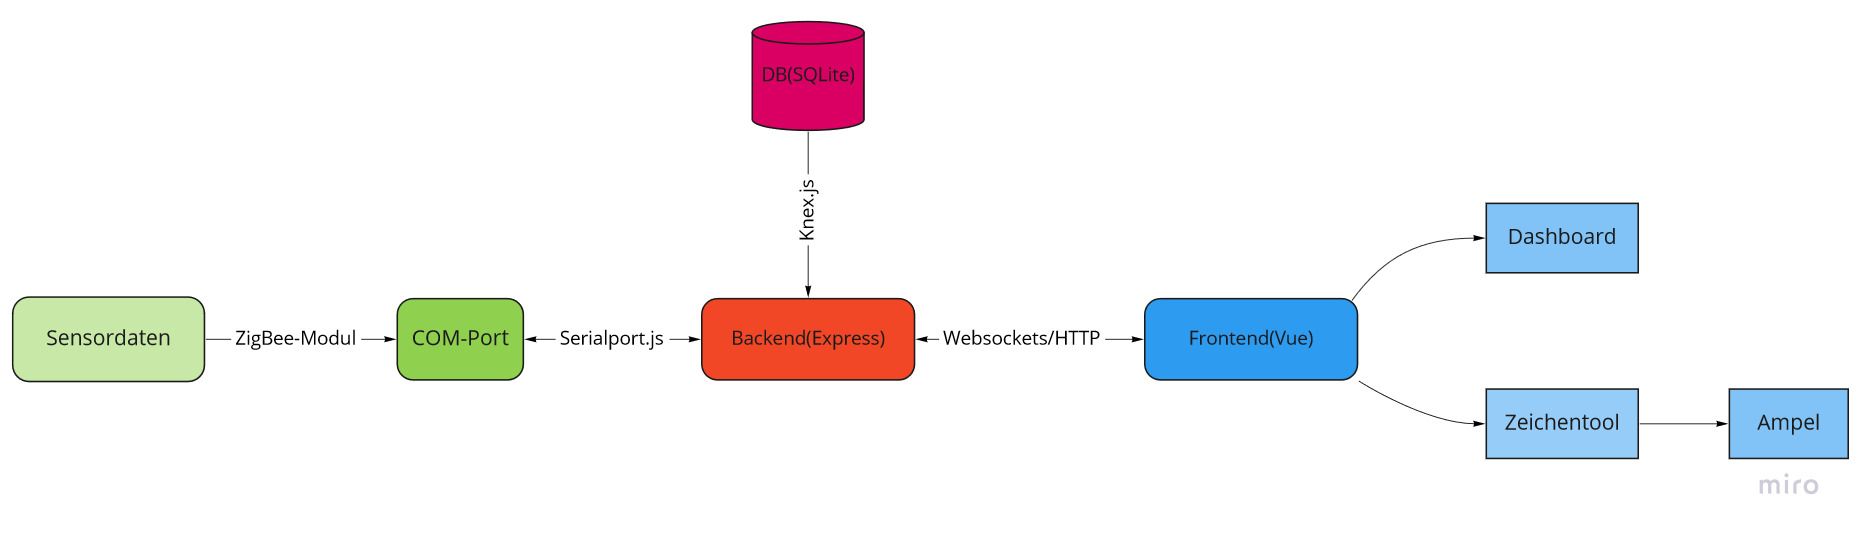
\includegraphics[scale=0.223]{images/DocArchitectureDiagram}
		\caption{Architekturdiagramm des Vorgangs zwischen Sensoren und Applikation}
		\label{img:DocArchitectureDiagram}
	\end{figure}
	\newpage
	\section{Aufgabenaufteilung} %kurze aufgabenteilung
	Zu Beginn des Projektes wurde entschieden die Aufgaben in zwei Teile aufzuteilen, einerseits in einen Sensorteil und andererseits in einen Applikationsteil. Es wurde festgelegt, dass Herr Merkert, Herr Just und Herr Glaesmann für die Einrichtung und Programmierung der Sensoren zuständig sind, während Herr Knez, Herr Nazlier und Herr Konieczka für die Einrichtung eines Servers und die Entwicklung der Applikation zuständig sind. 
		\subsection{Friedrich Just}
		\subsection{Stipe Knez}
			Herr Knez hat sich im Verlauf des Projektes um die korrekte Erstellung und Verwaltung der Mockdaten gekümmert. Darüber hinaus war er bei der Einrichtung des Backends samt der Datenbank beteiligt. Des Weiteren hat er sich um die Verbindung zwischen ZigBee-Modul und Backend über die COM-Port Schnittstelle und somit den Datenempfang gekümmert. Zuletzt hat er bei der Entwicklung des Dashboards mitgewirkt. 
		\subsection{Lucas Merkert}
			Aufgabe von Herr Merkert war die Programmierung des CCS811 Sensors, verschiedene administrative Aufgaben wie das organisieren von Meetings und Abgabe der Dateien und Recherche zum Thema Luftqualität in Innenräumen.
		\subsection{Achim Glaesmann}
		\subsection{Max-Rene Konieczka}
			Herr Konieczka war anfangs mit der Einarbeitung in Websockets beschäftigt um diese korrekt für die Übertragung der Daten zu verwenden. Zudem hat er Beihilfe bei der Integrierung von SerialPort.js geleistet, anschließend hat auch er sich wie Herr Knez und Herr Nazlier um die richtige Implementierung des Dashboards gekümmert, darunter auch Teile der Ampelindikation. 
		\subsection{Can Cihan Nazlier}
			Herr Nazlier hat sich zum einen um die Konfiguration der Programmierumgebung gekümmert. Dazu gehören die Erstellung eines GitHub-Repository und die Integrierung von Vue, einem JavaScript-Framework. Darüber hinaus hat er sich um die Integrierung einer Datenbank, die Implementierung des Zeichentools, anfangs in Form eines Prototypen, sowie einige Teile des Dashboards und der Ampelindikation gekümmert.
			\newpage
		
	\section{Luftqualität}%Lucas/Achim Friedrich
		Die Qualität der Luft setzt sich aus verschiedenen Faktoren zusammen. Für diese Projekt sind insbesondere die Faktoren Temperatur, Luftfeuchte, CO2 Gehalt und VOC (volatile organische Komponenten) wichtig, da wir mit den gegebenen Sensoren nur diese messen könne.
		\subsection{Luftfeuchte und Temperatur}
			Luftfeucht im allgemeinen bezeichnet die Menge an Wasserdampf die von der Umgebungsluft aufgenommen werden kann, bevor dieser kondensiert. Dabei unterscheidet man zwischen der absoluten, der maximalen und der relativen Luftfeuchte. Maximale Luftfeuchte bezeichnet hierbei den maximalen Wassergehalt in der Luft bevor das Wasser anfängt zu kondensieren. Die absolute Luftfeuchte gibt an wie viel Wasser sich derzeit in der Luft befindet und die relative Luftfeuchte gibt die Relation der beiden Größen in Prozent an. Die Luftfeuchte ist zudem stark von der Temperatur abhängig, dabei gilt: je höher die Temperatur der Luft desto größer die maximale Luftfeuchte und umgekehrt. Laut Inverter\cite{luftquali_inventer} ist für Wohn- und Arbeitsräume bei einer Temperatur von 20$^\circ$C eine Luftqualität von 40 - 60\% optimal. Bei zu geringer Luftfeuchte ($<$ 40\%) kann es u.A. zu Augen-, Haut-, und Schleimhautreizungen kommen. Bei Werten unter 23\% setzt Feuchtigkeitsverlust ein, der nicht über das Atmen kompensiert werden kann und es kann zu Stromschlägen bei Berührung mit Metall kommen. Zudem kann es zu Schäden an Bausubstanzen wie Holz u.ä. kommen. Bei zu hoher Luftfeuchte ($>$ 60\%) bildet sich schnell Schimmel welcher nicht nur die Bausubstanz schädigen kann sonder auch gesundheitliche Schäden nach sich ziehen kann. Überschreitet die Feuchtigkeit 80\% kann es zudem zur Vermehrung von Pilzen, Milben und anderen Parasiten kommen. Um dem Ganzen vorzubeugen, hilft es regelmäßig zu lüften.
		\subsection{CO2}
			Laut verschiedenen Quellen, u.A. dem Umweltbundesamt \cite{luftquali_bund_co2}\cite{luftquali_co2_corona}, gilt CO2 als Leitparameter um zu bestimmen wie viele Menschen sich in einem Raum aufhalten, vorausgesetzt es befinden sich keine weiteren CO2-Quellen in diesem Raum und kann somit auch als Indikator für die Ansteckungsgefahr durch Corona (SARS-COVID-19) verwendet werden. CO2 ist ein geruch- und farbloses Gas und ist mit einer Konzentration von 400ppm natürlicher Bestandteil der Umgebungsluft und wird vom Menschen hauptsächlich beim Ausatmen ausgestoßen, wie auch die Corona Viren. Das Umweltbundesamt \cite{luftquali_bund_co2_corona} hat hierfür eine Corona-Ampel eingeführt, welche hauptsächlich für die Anwendung in Klassenräumen vorgesehen ist. Dabei gilt eine Konzentration bis 1000ppm als gute Raumluft (grün), bei 1000 - 2000ppm schaltet die Ampel auf orange und bei über 2000ppm auf rot. Diese Ampel soll als Indikator dafür genutzt werden, das Lüftverhalten in einem Raum zu bestimmen. Zudem ist es wichtig die Sensoren möglichst mittig und auf Kopfhöhe, der sich im Raum befindenden Personen, zu platzieren. Allerdings kann man über die CO2 Konzentration nicht eine definitive Aussage über die Ansteckungsgefahr treffen, da die CO2 Konzentration auch durch verschiedene andere Faktoren beeinflusst wird im Gegensatz zum Ausstoß der Corona Viren. Hierbei spielen das Verhalten der Personen sowie das tragen einer Maske eine große Rolle. Betätigen sich die Personen in einem Raum schwerer körperlicher Arbeit (Fitnessstudio, Sport) so ist der CO2 Ausstoß sehr viel größer als wenn diese Personen nur Sitzen würden. Gleichzeitig verändert sich der Ausstoß der Viren nur wenig. Das gleiche gilt auch für das Sprechen und Singen. Beim Tragen einer Maske wird der Ausstoß von Viren deutlich gemindert, der Co2 Ausstoß bleibt aber gleich. Man kann also zusammenfassend sagen, das die CO2 Konzentration ein guter Leitparameter ist, jedoch die räumlichen Gegebenheiten auch eine große Rolle spielen.
		\subsection{VOC}
			Die volatilen organischen Komponenten (VOC) setzten sich aus verschiedenen Stoffen unterschiedlicher Emission zusammen. Meist betrachtet man hier organische Emissionsquellen wie Lebewesen, Baumaterialien wie Holz oder andere chemische Verbindungen. Diese Stoffe sind jederzeit in der Luft enthalten und in größeren Mengen schädlich für den Menschen und andere Lebewesen. Da VOC viele Schadstoffe zusammenfasst ist es schwer daraus eine konkrete Aussage über die Gesundheitlichen folgen zu machen. Schäden können laut Inverter \cite{luftquali_inventer} von Geruchsbelästigung, Augen- und Atemwegsreizung  über akute Vergiftungen bis hin zur Schädigung des Nervensystems, der Verstärkung von Allergien und dem Auslösen von Krebs reichen. Das Umweltbundesamt \cite{luftquali_bund_voc} unterscheidet hierbei sehr flüchtige und schwer flüchtige organische Verbindungen. Die Summe der Konzentrationen aller VOC ergibt den TVOC-Wert (total volatile organic compounds). Als Richtwerte existieren laut einem Bericht des Umweltbundesamts \cite{luftquali_bund_rw} der sog. Richtwert I und der Richtwert II. Diese Richtwerte gelten jedoch nicht für TVOC als Gesamtes sonder sind für die meisten enthaltenen Stoff festgelegt. Dabei bestimmt der Richtwert eine Grenze für die gilt, dass bei der Unterschreitung des Wertes auch bei lebenslanger Aussetzung keine gesundheitlichen Schäden zu erwarten sind. Im Gegensatz dazu stellt der Richtwert II eine Grenze dar, bei deren Überschreitung eine akute Gesundheitsgefahr besteht und ein unverzüglicher Handlungsbedarf besteht. Zudem wurde generell festgelegt, das die Konzentration der TVOC bei langfristiger Aussetzung nicht über 1 - 3 mg/m3 (ca 150 - 500ppb) überschritten werden sollte.
	\section{Lösungsansatz} %detaillierte beschreibung der einzelnen Aufgaben, probleme und Lösungen
		%TODO different subsections wer was wie gelöst hat und welche Probleme aufgetreten sind, dabei angeben welche Standards/werkzeuge/equipment genutzt worden sind
		\subsection{SHT21}
		\subsection{SCD41}
		\subsection{CCS811}
			Der CCS811 \cite{ccs_datasheet}ist ein Sensor von ams, der den äquivalenten CO2 (eCO2) Gehalt und den Gehalt der totalen flüchtigen organischen Verbindungen (TVOC) in der Luft messen kann. Dabei kann eCO2 von 400ppm bis 8192ppm, TVOC von 0ppb bis 1187ppb gemessen werden und ein Messintervall von 250ms, 1s, 10s, 60s festgelegt werden. Die Pin-Beschreibungen kann man in Abbildung \ref{img:ccs_pintable} sehen. Wichtig sind hiervon die Pins:
			\begin{itemize}
				\item VDD: Anschluss an 3,3V als Versorgungsspannung (min 1,8V)
				\item nWAKE: Anschluss an GND (active low), damit der Sensor durchgehend aktiv ist
				\item SDA: Data Anschluss für I2C, wird mit einem SDA Pin des Zigbee-Boards verbunden
				\item SCL: Clock Anschluss für I2C, wird mit einem SCL Pin des Zigbee-Boards verbunden
				\item GND: Ist nicht in der Tabelle angegeben, muss aber mit GND auf dem Zigbee-Board verbunden werden
			\end{itemize}
			\begin{figure}[!h]
				\centering
				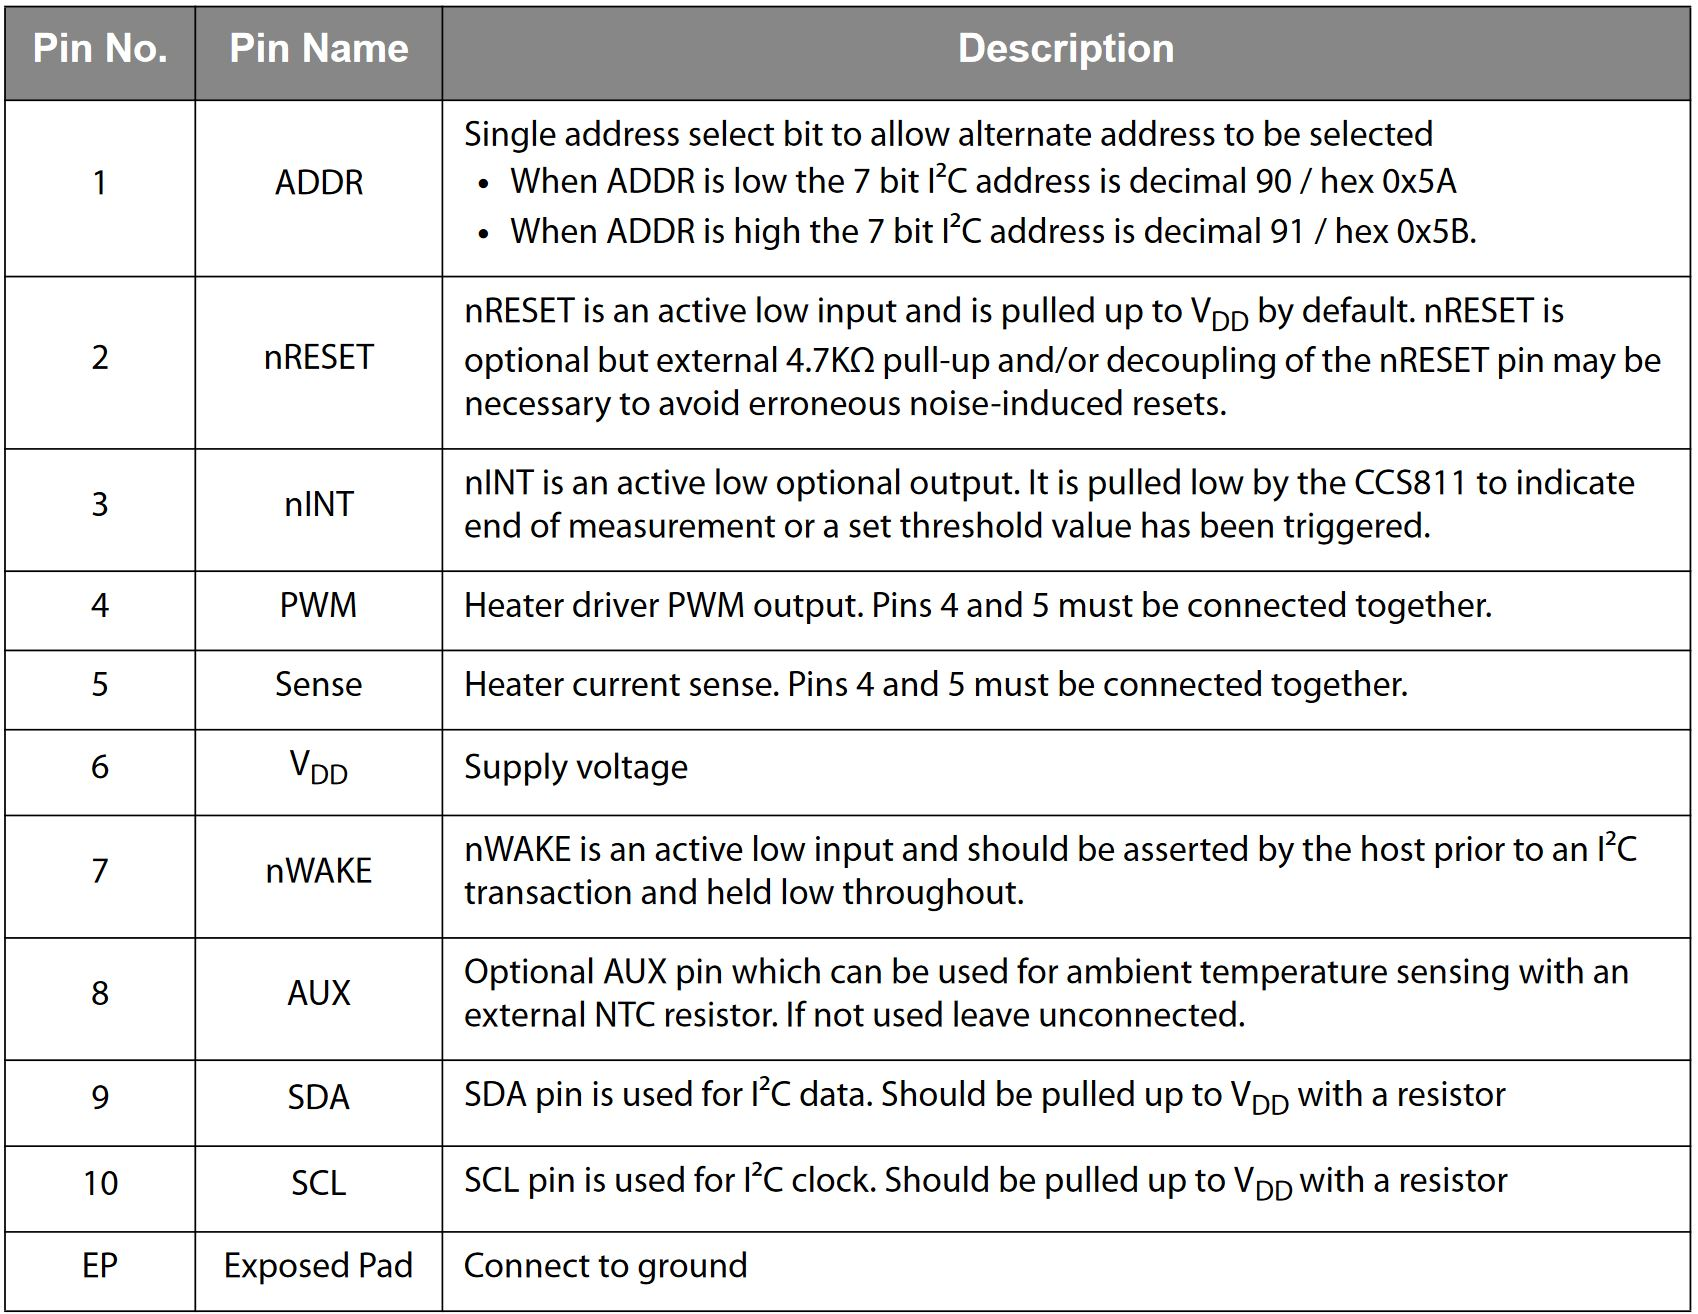
\includegraphics[scale=0.50]{images/ccs_pintable}
				\caption{Tabelle mit den Beschreibungen der Pins des CCS811}
				\label{img:ccs_pintable}
			\end{figure}
			In Abbildung \ref{img:ccs_zustandsdiagramm} ist das Zustandsdiagramm des CCS811 Sensors dargestellt. Zustände die nicht mit dem Sensor interagieren sind hier nicht dargestellt. Zu Beginn wird 2000 ms gewartet da der SCD41 Sensor entsprechende Zeit zum starten braucht. Die eigentliche Startzeit des CCS811 beträgt maximal nur 20ms. Der Zugriff auf den Sensor über den I2C-Bus spricht die Adresse 0x5A an, da der ADDR Pin nicht gesetzt ist. Im APP\_RESET\_CSS\_SW\_STATE wird mit 0xFF das SOFTWARE\_RESET\_REG angesprochen und der Befehl 0x11 0xE5 0x72 0x8A geschrieben. Dieser Befehl dient dazu einen versehentlichen Software Reset zu verhindern. Ist diese Sequenz geschrieben worden, befindet sich der Sensor im Boot mode. Zwischen den einzelnen I2C-Befehlen wird immer 1ms gewartet um sicherzugehen, das der Befehl richtig ausgeführt werden kann. Dies führt zwar zu einem erhöhten Zeitaufwand, ist jedoch unbedenklich, da der Messintervall 60 s beträgt und somit genügend Zeit zur Verfügung steht. Im nächsten Schritt wird das HW\_ID\_REG angesprochen und im darauf im folgenden Zustand auch ausgelesen. Hierbei ist wichtig, dass die HW\_ID 0x81 ist. Im APP\_CCS\_CHANGE\_TO\_APPSTATE\_STATE wird mit dem Befehl 0xF4 zurück in den Appstate gewechselt. Nun wird das MEAS\_MODE\_REG 0x01 angesprochen und der Befehl 0x30 geschrieben. Dieser Befehl setzt den Messintervall auf 60s, welcher den geringsten Stromverbrauch hat. Zum Testen der Applikation wurde hier ein kürzerer Intervall gewählt. Zudem werden keine Interrupts gesetzt die feuern würden wenn Daten vorhanden wären. Um zu überprüfen ob die Messung funktioniert, wird nun 60s gewartet und dann das STATUS\_REG 0x00 überprüft, ob Daten vorhanden sind. Ist dies der Fall, ist das 3. Bit gesetzt. Falls ein Fehler auf dem I2C-Bus oder dem Sensor aufgetreten ist, könnte man dies über das 0. Bit feststellen und im Register 0xE0 auslesen. Sind Daten zum abrufen bereit, werden die Sensoren SHT21 und SCD41 initialisiert. Dabei wird auch der Messtimer von 60s gestartet. Sind diese 60s abgelaufen, so wird das ALG\_RESULT\_DATA\_REG 0x02 angesprochen in dem die bereits berechneten Daten der Messung bereit liegen. Diese werden als 4 Byte ausgelesen, wobei die Bytes 0 und 1 den eCO2 Wert beinhalten und Byte 3 und 4 den TVOC Wert. Eine Umrechnung der Daten ist nicht nötig, da diese bereits der Sensor selbst umrechnet und somit im richtigen Format ausgelesen werden können.
			\begin{figure}[!h]
				\centering
				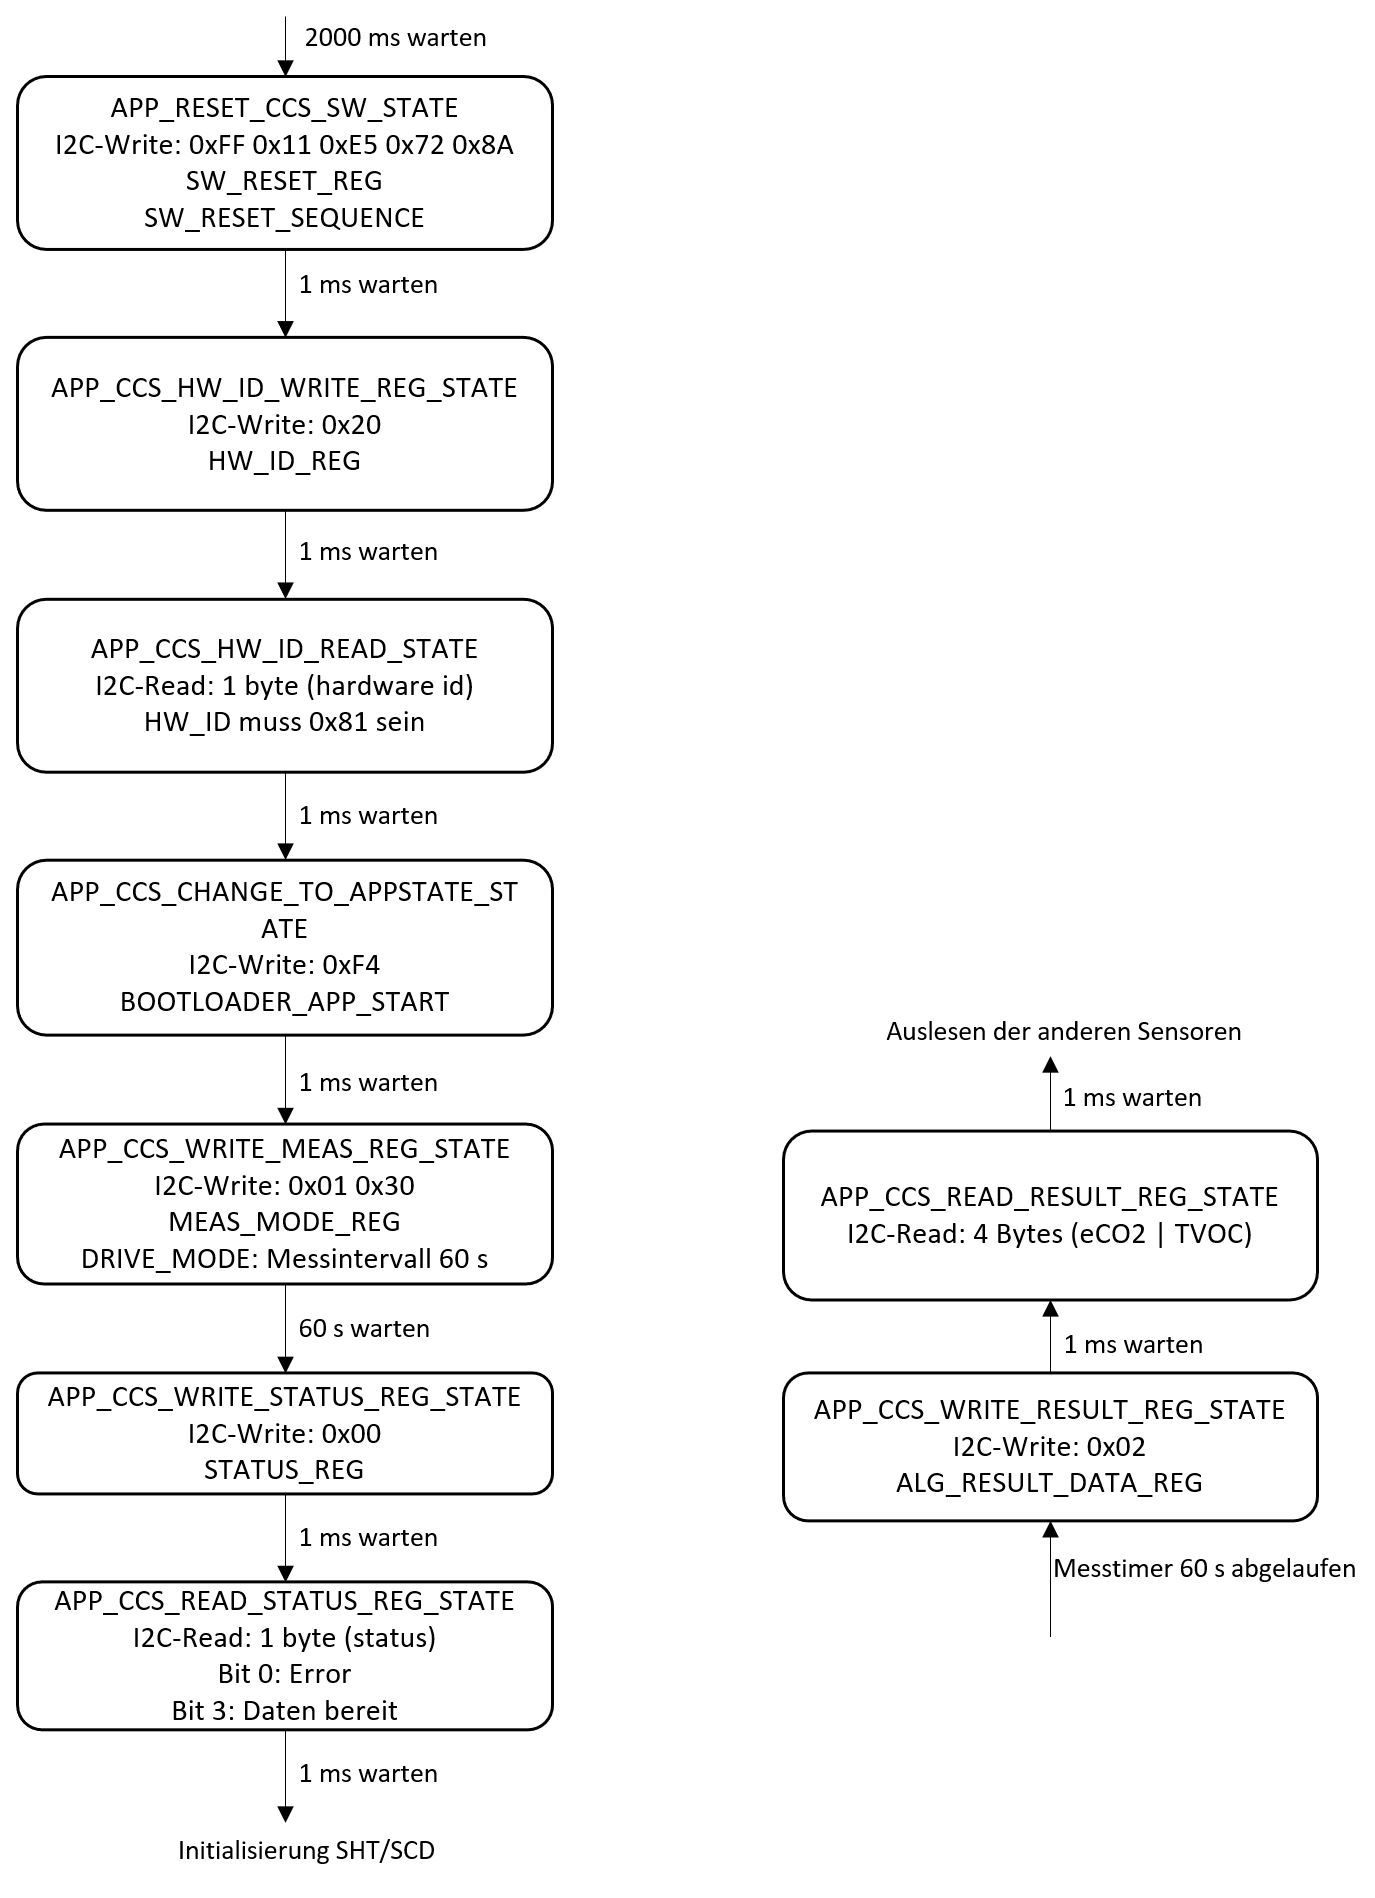
\includegraphics[scale=0.30]{images/ccs_zustandsdiagramm}
				\caption{Zustandsdiagramm des CCS811 Sensors, rechts: Initialisierung, links: Auslesen der Werte}
				\label{img:ccs_zustandsdiagramm}
			\end{figure}
				\subsubsection{Probleme bei der Programmierung des CCS811}
					Da sich der CCS811 in seiner Funktionsweise von den anderen beiden Sensoren unterscheidet, war es zu Anfang schwierig einen richtigen Ansatz zu bekommen. Vor allem das Wechseln in den Bootmodus war erst nach der Erläuterung in der Vorlesung klar und damit auch nachvollziehbarer. Zudem haben teilweise die Funkmodule nicht richtig Funktioniert, da entweder überhaupt nichts über die UART ausgegeben werden konnte oder die bei einem I2C-Befehl der Callback mit Error zurück gekommen ist. Nachdem wir den Code mehrmals auf Richtigkeit der Befehle und Ablauf überprüft haben, haben wir das ZigBee-Board ausgewechselt und das Messen hat ohne Probleme funktioniert. Was dabei der genaue Fehler war ist uns nicht bekannt. Zudem war die Funktion der Pins nWAKE und ADDR zu Anfang nicht klar. Der nWAKE Pin ist dafür da damit der Sensor aktiv ist und muss dafür auf low gezogen werden. Also haben wir diesen and GND angeschlossen und somit ist der Sensor durchgehend aktiv. Der ADDR Pin gibt an ob die I2C-Adresse des Sensors 0x5A oder 0x5B ist. Da der ADDR Pin nicht angeschlossen ist, ist die I2C-Adresse 0x5A.
				\subsubsection{Funktionsweise des CCS811}
					Der CCS811 Sensor ist ein Metalloxid Sensor, der mittels eines anorganischen Metalloxid-Halbleiters, welcher mit der Zielsubstanz (Hier CO2 und VOC) reagiert und dadurch seinen Widerstand ändert. Aus der Änderung des Widerstands kann dann die Konzentration der Zielsubstanzen ermittelt werden \cite{wiki_gassensor}. Laut dem Datenblatt des Sensors wurde hierfür die von ams entwickelte "micro-hotplate technologie" verwendet. Probleme bei diesem Verfahren ist das Aussondern der Zielsubstanz und das Verhindern der Beeinflussung durch andere Substanzen (andere Gase) oder Einflüsse (Luftfeuchte). Die Beeinflussung durch andere Substanzen kann durch die Wahl des Metalloxids eingeschränkt werden, andere Einflüsse können wenn überhaupt nur durch ständige Anpassung der Berechnung ausgeglichen werden. Um eine Substanz, hier z.B. CO2 zu messen, reagiert das Metalloxid mit dem Gas. CO2 ist dabei ein oxidierendes Gas, gibt also Sauerstoff an das Metalloxid ab und verringert dadurch die Leitfähigkeit des Halbleiters. In Abbildung \ref{img:metalloxid_sensor} kann man dazu einige Beispiele sehen.
					\begin{figure}[!h]
						\centering
						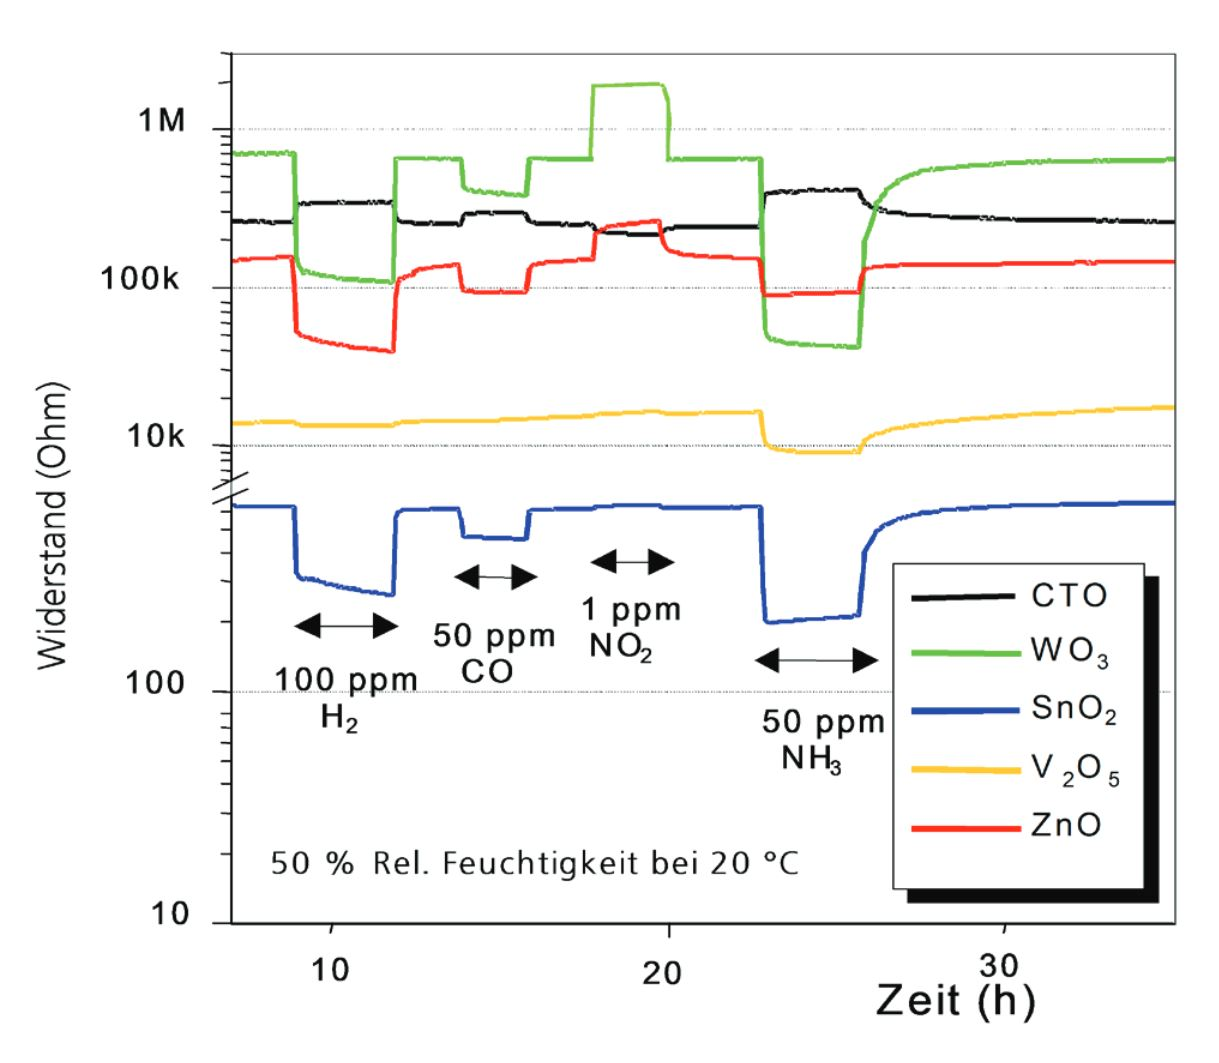
\includegraphics[scale=0.30]{images/metalloxid_sensor}
						\caption{Verschiedene Metalloxide und die Veränderung des Widerstands durch die Reaktion mit verschiedenen Gasen\cite{metalloxidsensor}}
						\label{img:metalloxid_sensor}
					\end{figure}
					%TODO wikipedia als quelle?!
					
					
			\subsection{Messung der Eingangsspannung}
			Für die Messung der Eingangsspannung wurde der Analog-to-Digital Converter genutzt, auch ADC genannt, welcher sich auf dem ATmega256RFR2 befindet. Dieser wandelt analoge Signale in digitale um. Für die Eingangsspannung muss der ADC0-Pin ausgelesen werden. Hierfür nutzt man die Register, die im Datasheet S.465 beschrieben sind. Die Bits von MUX5:0 werden auf 0 gesetzt (Referenz)Z.4-5. Des Weiteren wird die interne Referenzspannung von 1.5V im ADMUX Register ausgewählt. Dafür setzt man das REFS1 Bit auf eins und REFS0 auf Null (Referenz)(Z.4). Jetzt wird noch der ADC eingeschaltet, indem man im ADCSRA Register das ADEN Bit auf Eins stellt. Danach startet man die Messung, indem man im ADCSRA Register das ADSC Bit auf Eins stellt (Referenz)(Z.8). Wenn die Messung erfolgt ist, wird das ADSC Bit auf Null gestellt und das Ergebnis im ADCW Register gespeichert. Diesen Wert wird mit sechs multipliziert, um den Messwert in Millivolt zu erhalten. In Listing (ATMEGADATASHEETT REFERENCE S. 465)
			Es werden mehrere Werte gemessen, um so einen genaueren Durchschnitt zu berechnen.
			
			\begin{lstlisting}[language=C,frame=single, caption = Delay Timer, label = delay_timer] 
				static uint16_t vcc_read(void){
					uint32_t adcval = 0;
					
					ADMUX  |= (1<<REFS1)|(0<<REFS0)|(0<<MUX4)|(0<<MUX3)|(0<<MUX2)|(0<<MUX1)|(0<<MUX0);			ADCSRB |= (0<<MUX5);
					ADCSRA |= (1<<ADEN); // ADC einschalten
					for(uint16_t i=0; i<NUM_MESS_ADC; i++){
						ADCSRA |= (1<<ADSC); // start messung
						while (ADCSRA&(1<<ADSC)){
						}
						adcval += ADCW;
					}
					ADCSRA &= ~(1<<ADEN); // ADC ausschalten
					return (((adcval)/NUM_MESS_ADC) * 6);
				}
				
			\end{lstlisting}
			
			
			\subsection{Datenübertragung}
			Bei der Datenübertragung wurde entschieden, alle Sensordaten in einem uint8\_t Array zu versenden. Dieses Array ist somit immer 44 Byte lang. Die verschiedenen Werte sind durch Semikolons getrennt. Es folgt die Liste mit allen Werten aus dem Array mit passender Umrechnung und Maßeinheit:
			\begin{enumerate}
				\item ID es Mikrocontrollers		
				\item SHT21 Temperatur				(Wert/100 in $^\circ$C)
				\item SHT21 Relative Luftfeuchte	(Wert/100 in \%)
				\item SCD41 Temperatur				(Wert/100 in $^\circ$C)
				\item SCD41 Relative Luftfeuchte	(Wert/100 in \%)
				\item SCD41 CO2						(Wert in ppm)
				\item CCS811 eCO2					(Wert in ppm)
				\item CCS811 TVOC					(Wert in ppb)
				\item Spannung 						(Wert in Millivolt)
			\end{enumerate}
			\begin{figure}[!h]
				\centering
				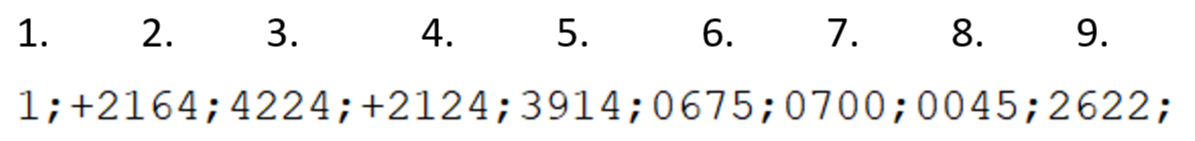
\includegraphics[scale=0.60]{images/data_example}
				\caption{Beispiel Messdaten Array}
				\label{img:data_example}
			\end{figure}
			
			
			Wenn alle Werte im Array sind, müssen diese in die Payload übertragen werden. Mit diesem Befehl APS\_DataReq(\&datareq); werden die Daten an den Koordinator gesendet.
			
			\subsection{Netzwerkaufbau}
			\subsubsection{Aufbau}
			In dem Netzwerk gibt es drei verschiedene Rollen. 
			
			\begin{enumerate}
				\item Der Router leitet die ankommenden Daten an den Koordinator oder an andere Router weiter. 
				\item Der Koordinator ist dafür verantwortlich, dass das ZigBee-Netzwerk startet. Er fungiert auch als Router.
				\item Das Endgerät kommuniziert nur mit dem Router und Koordinator. 
			\end{enumerate}
			
			In der Header Datei configurations.h müssen verschiedene Voreinstellungen vorgenommen werden. 
			
			\begin{enumerate}
				\item Die Rolle des Gerätes in der Variablen CS\_DEVICE\_TYPE
				\item Der "Unique identifier" auch genannt CS\_UID. Dieser ist 64-Bit lang. Der Koordinator hat die UID 0x0700000A01LL.
				Die Endgeräte beginnen bei der UID 0x0700000A03LL und jedes weitere wird die letzte Stelle um eins erhöht.
				
				\item Die eindeutige Netzwerk PAN-ID. Diese ist 64-Bit lang und wir in der Variablen CS\_EXT\_PANID mit dem Wert 0x1AAAAAAAAAAACA07LL definiert.
			\end{enumerate}
			
			
			NETZWERK AUFBAU ERKLÄRUNG FEHLT
			
			
			\begin{figure}[!h]
				\centering
				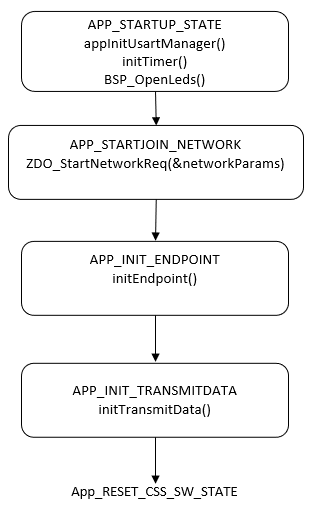
\includegraphics[scale=0.60]{images/Netzwerkaufbau}
				\caption{Beispiel Messdaten Array}
				\label{img:Netzwerkaufbau}
			\end{figure}
			
			 
			\subsubsection{Probleme beim Zusammenfügen der Sensoren und des Netzwerkes}
			Als der Code für die Sensoren zusammen gefügt wurde, hat der SCD41 und der CSS811 plausible Werte ausgegeben. Der SHT21 hingegen hat zu hohe Werte geliefert. Wenn man eine Batterie an das Endgerät angeschlossen hat, wurden falsche Messdaten empfangenen. Bemerkenswert war, dass nur der SCD41 falsche Werte liefert. Später bei dem Messen der Spannung hat sich herausgestellt, dass die minimale benötigte Spannung von 2,4 Volt unterschritten worden ist. Deshalb konnte der Sensor nicht korrekt ausgelesen werden. Darum wurden die aktuellen Werte nicht mehr aktualisiert und immer die gleichen Wert versendet. Wenn das Gerät neu gestartet worden ist, konnte der Sensor nicht initialisiert werden und es wurde immer -45.00 $^\circ$C und Nullen bei der Luftfeuchte und CO2 gesendet.
			
			
			\subsection{Messdaten Auswertung}
			Diese Messdaten wurden im Innen- und Außenbereich getestet und mit einem anderen Temperatur, Luftfeuchtigkeits und CO2 Sensor von der Firma NETATMO verglichen und ähnliche Werte wurden festgestellt Bilder....................................
			Hier wurden sich vier Zeitpunkte ausgesucht und die Messwerte beider Geräte verglichen
			
			
					
			\subsection{Serverimplementierung}
				Wie eingangs erwähnt, wird das Express.js Framework benutzt um unsere Webanwendung aufzubauen.... vllt doch nicht nochmal erwähnen
			
			\subsection{Zeichentool}
				\subsubsection{Aufbau und Funktionsweise}
				Die einzelnen Komponenten des Zeichentools wurden mit Vue erstellt. Diese bestehen aus HTML und CSS Elementen sowie einem Skript-Teil, in welchem jegliche Funktionalitäten in Java- oder Typescript programmiert werden können. Die Buttons sind beispielsweise im HTML-Abschnitt eingebettet und Funktionen zur Realisierung des Hinzufügens von Sockets für die Live-Daten Übertragung oder eine Anknüpfung an die Datenbank um gezeichnete Räume abspeichern zu können, sind im Skript-Abschnitt implementiert. 
				Für das Zeichentool wurde zunächst ein Prototyp geschrieben, um zu testen inwiefern man Räume einzeichnen können soll. Nachdem dieser erstellt worden war, wurde auf diesem Prototyp aufgebaut und das eigentliche Zeichentool implementiert. Mit einem Doppelklick lassen sich Punkte auf die Leinwand platzieren, sobald ein zweiter Endpunkt hinzugefügt wurde, entsteht eine Linie zwischen diesen Punkten. Erst nachdem ein geschlossener Raum gezeichnet und ihm ein Name gegeben wurde, kann man diesen permanent speichern und anzeigen lassen. Wenn man den Button \textbf{Show Rooms} anklickt, wird in einem kleinen Fenster jeder Raum angezeigt, welcher gespeichert wurde. In dieser Übersicht gibt es drei weitere Funktionen, es können Sensoren in den verschiedenen Räumen platziert werden, überflüssige Räume können wieder entfernt und es kann über den Info-Button eine Tabelle angezeigt werden lassen, welche die Zahlenwerte der Sensoren anzeigt.\newline Auch die Ampelindikation ist im Zeichentool verwirklicht worden. Wenn man einen Sensor in einen Raum hinzufügt, kann dieser frei innerhalb des Raumes bewegt werden. In diesem Fall ist der Sensor selbst die Ampelindikation. Abhängig von der CO2-Konzentration, ändert die Indikation die Farbe von grün auf gelb und von gelb auf rot. 
				\subsubsection{Probleme beim Zeichentool}
		 		Wenn ein Raum gezeichnet und nicht direkt abgespeichert wird, kann man die Eckpunkte des Raumes auswählen und dadurch weiterhin durch die Leinwand bewegen. Somit können Räume möglicherweise noch nachjustiert werden. Wenn man allerdings unbeabsichtigt die Linie auswählt, wird diese von den Punkten getrennt. Dies hat den Grund, dass die Linie dynamisch implementiert wurde um dem User eine Nachjustierung zu ermöglichen. Wäre die Linie statisch eingebunden worden, könnte man sie nach der Entstehung zwischen zwei Punkten in keinerlei Weise beeinflussen. Der Anwender kann diesen Fehler allerdings ganz einfach wieder beheben, indem einer der Punkte ausgewählt und bewegt wird. \newline Ein weiterer Punkt wäre eine Verzögerung bei der Informationstabelle, wenn der Info-Button betätigt wird. Die Tabelle zeigt zunächst keine Werte an, diese werden erst nach 1 Minute geladen. 
			
			\subsection{Dashboard}
			\subsubsection{Funktionsweise}
			Das Dashboard ist hauptsächlich dazu da, die ankommenden Sensordaten visuell darzustellen. Es besteht aus 4 Liniendiagrammen, die die Werte von Temperatur, relativer Feuchtigkeit, CO2 und TVOC anhand eines Liniengraphen anzeigen. Der Anwender hat die Möglichkeit verschiedene Zeiten einzustellen, somit kann er die Daten der vergangenen letzten 6, 24 und 168 Stunden aufrufen.
			Wenn einer der Zeit-Buttons benutzt wird, kann man für die nächsten drei Sekunden keine weitere Eingabe tätigen und werden erst nach diesem Zeitraum wieder freigeschaltet. Es braucht nämlich 3 Sekunden, bis die Daten vom Backend im Frontend geladen werden.\newline Die Y-Achse passt sich entsprechend den Werten der übertragenen Daten an. Die X-Achse hingegen besteht aus genau 120 Ticks, abhängig davon ob 6, 24 oder 168 Stunden angegeben werden, passen sich die Sensorwerte an die 120 Ticks an. Das bedeutet, wird die 6 Stunden Option ausgewählt, werden Daten in 3 Minuten Takten angezeigt, bei 24 Stunden sind es 12 Minuten Takte und bei 168 Stunden bzw. 1 Woche sind es 84 Minuten Takte. Der Grund für die statische Anzahl an Ticks ist, dass es bei einer höheren Zahl zu Performance-Einbrüchen kommen würde und die Anwendung dadurch langsamer arbeitet.\newline
			\subsubsection{Aufgetretene Probleme}
			Zunächst war festgelegt, dass die JavaScript-Library D3.js verwendet wird um die graphische Darstellung der Sensordaten zu realisieren. Diese enthält Funktionen um verschiedenste Diagramme zu erstellen. Die Funktionen manipulieren HTML-Elemente, dadurch können z.B. einerseits deren Größe und Breite eingestellt oder andererseits können komplett neue HTML-Elemente hinzugefügt werden. Das Erstellen von vier verschiedenen Liniendiagrammen und einer Ampel war zunächst schnell abgeschlossen. Nach dieser Erstellung wurde ein Socket implementiert um zu überprüfen, ob die Sensordaten im Dashboard ankommen, was im Anschluss auch der Fall war. Allerdings ist hier ein Problem hervorgekommen.\newline
			Die Sensorwerte sollten als Y-Koordinate und die dazugehörige Zeit als X-Koordinate angezeigt werden. Zwar gibt es in D3.js eine eigens dafür integrierte scaleTime-Funktion um eine Zeitachse zu erstellen, aber durch die Zeiteinheit konnte nun kein Graph angezeigt werden. Dies hatte den Grund, dass zu diesem Zeitpunkt kein Zeitwert von der Datenbank übertragen wurde. Für dieses Problem konnte keine direkte Lösung hinsichtlich der Implementierung gefunden werden, daher wurde kurzfristig entschieden auf die Chart.js-Library umzusteigen. Diese bietet beispielsweise fertige Diagramme an, in welchen man lediglich personalisierte Werte hinzufügen kann.\newline 
			Während der Implementierung ist hervergekommen, dass wenn der Anwender zu schnell zwischen dem Zeichentool- und Dashboardfenster hin und her wechselt, kann es passieren das keinerlei Graphen bzw. Daten im Dashboard angezeigt werden, da diese nicht fertig geladen wurden. Dies kann allerdings mit einem erneutem Neuladen der Dashboardseite wieder behoben werden. %Vllt noch ein bisschen zur Implementierung
			\subsection{COM-Port \& Mockdaten}
			
			\subsubsection{Mockdaten}
			Zu Beginn des Projekts wurde zur Simulation von Sensordaten ein Python-Programm genutzt. Der Sinn dahinter war, auch Gruppenmitgliedern, die sensorisch nicht voll ausgestattet sein konnten, Daten zur Verfügung zu stellen, um die Anwendung im Back- und Frontend testen zu können. Auch sollte durch die Verwendung von Mockdaten das Back- und Frontend-Team nicht auf die Vollendung der Programmierung der ZigBee Module durch das ZigBee-Team warten müssen, um die Applikation zu testen.\newline			
Um die Idee in die Tat umzusetzen, wurde die “pySerial” API genutzt. Das Programm erstellte Datensätze und schickte diese an eine COM-Schnittstelle des Computers. Da zu diesem Zeitpunkt noch die Idee im Raum war, dass die Daten als JSON-string von den ZigBee Modulen an den Computer geschickt werden sollen, wurden die Datensätze im Python-Programm als JSON-Strings formatiert und abgeschickt.\newline
Im weiteren Verlauf des Projekts wurde sich, was das Format der übertragenen Daten angeht, umorientiert. Es wurde klar, dass das Verhältnis zwischen Aufwand und Nutzen bei Nutzung eines JSON-Formats nicht gut genug war. Deshalb wurde sich dazu entschieden, die Daten in Form eines einfachen Strings, in dem die Daten jeweils durch ein Semikolon getrennt werden, an den Computer zu  übertragen (Abb. \ref{img:data_format}). Des Weiteren wurde, um eine realitätsgemäße Datenübertragung simulieren zu können, die Verwendung des Python-Programms verworfen und auf ein ZigBee C-Programm zur Datensimulation gewechselt. Hierzu wurde ein ZigBee Modul darauf programmiert, einen String im zuvor erwähnten Format an die COM-Schnittstelle in einem vordefinierten Intervall zu schicken. Die Intervalllänge wurde dabei aus Zeiteffizienzgründen auf 10 Sekunden gesetzt.
					\begin{figure}[!h]
						\centering
						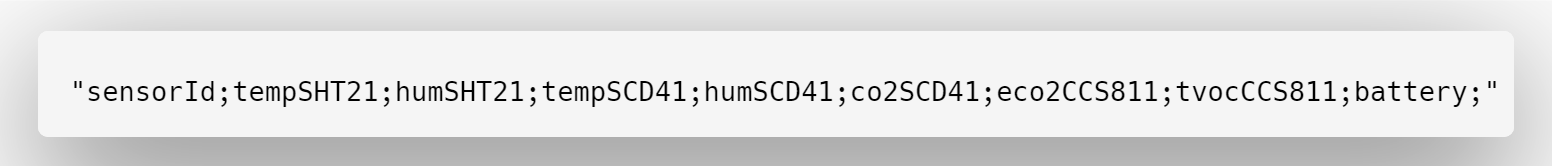
\includegraphics[scale=0.223]{images/data_format}
						\caption{Format in dem die Datensätze übertragen werden}
						\label{img:data_format}
					\end{figure}

			\subsubsection{Kommunikation über den COM-Port}
			Die Kommunikation zwischen Computer (Backend) und dem ZigBee Modul und somit auch den Datenempfang und die Datenverarbeitung haben wir mit Hilfe des Node.js Packages “SerialPort” realisiert.\newline
Im Backend wird zur Kommunikation mit dem ZigBee Modul ein SerialPort-Objekt genutzt. Dieses wird erstellt, sobald der Anschluss eines ZigBee Moduls an den Computer von unserer Anwendung registriert wird.\newline
Das erstellte SerialPort-Objekt benötigt bei der Erstellung einige Informationen über das angeschlossene Gerät, um einen reibungslosen Datenempfang und eine daran anschließende Verarbeitung zu ermöglichen. Dabei handelt es sich vor Allem um den Port, über den das Gerät kommuniziert und die verwendete Baudrate. Da der verwendete COM-Port von Nutzer zu Nutzer variiert, musste sich überlegt werden, wie eine automatische Erkennung des richtigen COM-Ports implementiert werden kann. Eine manuelle Eingabe des Namens des richtigen COM-Ports durch den Nutzer war nicht gewollt, da dies auf Kosten des Nutzerkomforts geschehen würde. \newline 
Da das SerialPort Package keine Funktion zur Erkennung des richtigen COM-Ports zur Verfügung stellt, musste sich überlegt werden, wie dies mit den vorhandenen Mitteln umgesetzt werden könnte. Die Umsetzung ist durch die Entwicklung und Implementierung einer Funktion gelungen, die den richtigen Portnamen ermittelt. Das Vorgehen ist dabei wie folgt:\newline 
Die Funktion erstellt eine Liste aller verfügbaren COM-Ports des Computers und iteriert über alle (Abb. \ref{img:getPortName}, Z.4-9). Bei jedem Port wird dabei überprüft, welchen manufacturer und welche vendorId das angeschlossene Gerät besitzt. Wenn dabei das angeschlossene Gerät den manufacturer “FTDI” und die vendorId “0403” hat, dann handelt es sich bei dem angeschlossenen Gerät um ein ZigBee Modul und es wird der entsprechende Name des Ports, über den das Modul kommuniziert, in die Variable “portName” gespeichert.\newline
Durch einen in den Server eingebauten Timer, der immer wieder getPortName() in einem Intervall von einer Sekunde aufruft, bis ein ZigBee Modul an den Computer angeschlossen wird, wird getPortName() erneut aufgerufen und führt dabei diesmal den else-Teil der Funktion aus. Anschließend wird das Aufrufintervall zurückgesetzt und somit vorerst ein erneuter Aufruf ausgeschlossen. Daraufhin wird dann “portName” bei der Erstellung des SerialPort-Objektes mitgegeben, womit dann die Grundlage für den Datenempfang gebildet wird (Abb. \ref{img:getPortName}, Z.13). Für den Fall, dass dies erfolgreich ist, erkennt ein Event-Listener dies (Abb. \ref{img:getPortName}, Z.14-16) und bestätigt den Erfolg durch eine Konsolenausgabe. Für den Fall, dass es fehlschlägt, erkennt dies ein weiterer Event-Listener (Abb. \ref{img:getPortName}, Z.17-22) und gibt eine entsprechende Meldung in der Konsole aus und wartet auf einen erneuten Verbindungsversuch. Im Erfolgsfall wird dann des Weiteren die Funktion listen() aufgerufen (Abb. \ref{img:getPortName}, Z.23), welche dann auf eingehende Daten wartet und diese dann dementsprechend verarbeitet.\newline
Wie zuvor erwähnt, wird getPortName() immer wieder aufgerufen, bis ein ZigBee Modul erkannt und somit die Variable “portName” gefüllt wird. Dies kann unmittelbar nach Serverstart oder auch in Folge eines Aussteckens des Moduls der Fall sein. Für den Fall, dass eine bestehende Verbindung zwischen dem Modul und dem Computer getrennt wird, wurde in den Else-Teil von getPortName() noch ein weiterer Event-Listener integriert(Abb. \ref{img:getPortName}, Z.24-31). Nach dem Einrichten des Datenempfangs durch listen(), sorgt die asynchrone Funktion dafür, dass während einer bestehenden Verbindung von Modul und Computer direkt auf den Fall eines Verbindungsabbruchs reagiert werden kann. Wenn vom Port ein “close” Event emittiert wird, das durch einen Verbindungsabbruch ausgelöst wurde, wird die Variable “portName” automatisch wieder geleert und das einsekündige Intervall tritt wieder in Kraft, wodurch wieder auf ein erneutes Verbinden des Moduls mit dem Computer gewartet wird.  
						\begin{figure}[!h]
							\centering
							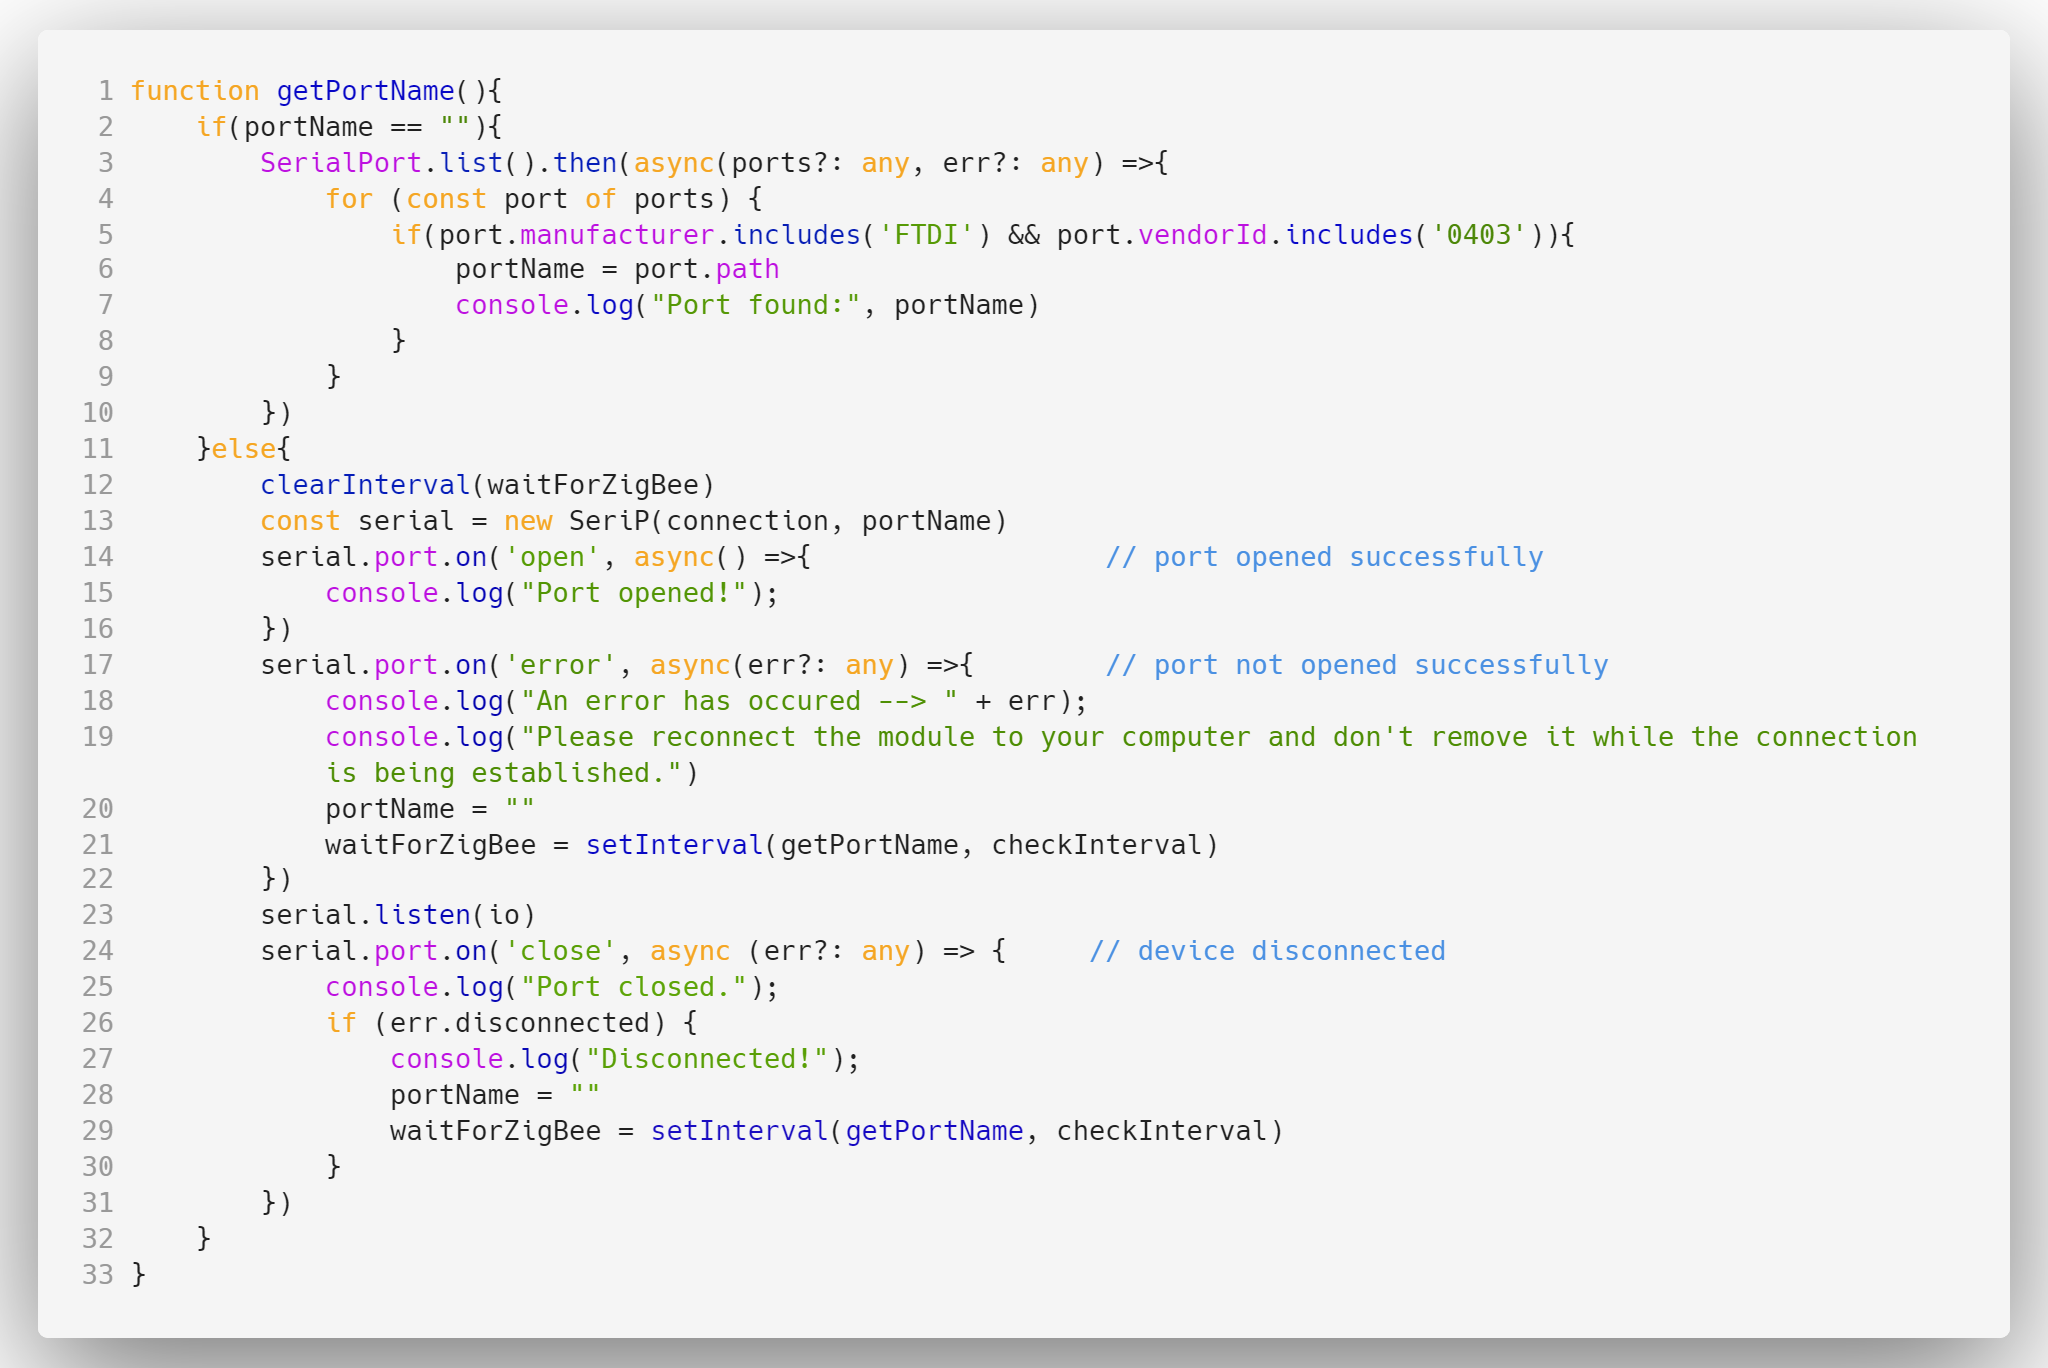
\includegraphics[scale=0.18]{images/getPortName}
							\caption{Funktion “getPortName()”}
							\label{img:getPortName}
						\end{figure}

			\subsubsection{Aufgetretene Probleme}
			Ein anfängliches Problem stellte der Absturz des Servers direkt nach seinem Start dar, wenn bei Serverstart kein Modul verbunden war. Der Grund dafür war, dass zu diesem Zeitpunkt der Name des COM-Ports hardcoded war und die Anwendung dabei versucht hat, einen Port anzusprechen, an dem kein Gerät verbunden ist. Dies führte dann zwangsläufig zum Absturz des Servers. Außerdem kam es bei einem Verbindungsabbruch zwischen Modul und Computer dazu, dass der Server zwar weiterlief, aber ein erneutes Verbinden des Moduls nicht zur erneuten Erkennung der Verbindung führte und auch kein Datenempfang im Backend stattfand.\newline
Diese beiden Probleme konnten durch die Implementierung der automatischen COM-Port Erkennung in Form von getPortName() in Verbindung mit dem Timer gelöst werden.\newline
Ein weiteres Problem, das nach der Lösung der beiden vorherigen auftrat, war, dass sich ein Serverabsturz provozieren ließ, wenn man das Modul vom Computer getrennt hat, während die Verbindung zum Modul initialisiert wurde und noch nicht abgeschlossen war. In der Praxis bedeutet das, dass man das Modul etwas mehr als eine Sekunde nachdem man es angesteckt hat, wieder absteckt. Der technische Hintergrund dabei ist, dass unsere Anwendung sobald ein ZigBee-Modul angesteckt wird, den richtigen Port erkennt und daraufhin dazu übergeht ein SerialPort-Objekt zu erstellen. Bei der Erstellung des SerialPort-Objektes wird dann versucht, den angegebenen Port zu öffnen. Dies ist aber nur möglich, wenn es ein angeschlossenes Gerät gibt, das auf diesen Port zugreift. Wenn wir nun, noch bevor das SerialPort-Objekt erstellt wird, die Verbindung zwischen Modul und Computer unterbrechen, kann der Port nicht geöffnet werden. Dieser Fehler löste den Serverabsturz aus.\newline  
Dieses Problem ließ sich durch den Einbau eines bestimmten Event-listeners (Abb. \ref{img:getPortName}, Z.17-22), der bei der Erstellung eines SerialPort-Objektes darauf wartet, dass ein “error” Event emittiert wird, beheben. Bei der erfolgreichen Erstellung eines solchen Objektes wird nämlich ein “open” Event emittiert und bei einem Fehlschlag ein “error” Event. Wenn nun ein “error” Event emittiert wird, wird der Fehler in der Konsole geloggt und auf ein erneutes Anschließen des Moduls gewartet. Somit wird ein Absturz des Servers durch das abfangen des Fehlers verhindert und ein Warten auf eine erneute Verbindung durch wiederholtes Ausführen der getPortName() Funktion ermöglicht.

			\subsection{Installationsdatei}
			Alles bisherige wurde in Express.js gebündelt und in zwei PowerShell-Skripte unterteilt. Einmal wird das kompilierte Frontend mit Electron, und das kompilierte Backend in Express.js gestartet.
			Es konnte keine EXE.-Datei erstellt werden, da die Nodeversion vom Serialport.js, was verwendet wurde um die Kommunikation mit den COM-Port Schnittstellen herzustellen, und die serverseitige Nodeversion verschieden und daher nicht kompatibel waren. Auch Electron war von der Versionsinkompatibilität betroffen. 
			
	\section{Auswertung des Testlaufs}
			
	\section{Ausblick und Erweiterungsmöglichkeiten}
		\subsection{Optimierung für Batterien}
		\subsection{Genauere Bestimmung der Werte des CCS811}
			Wie bereits angesprochen ist der Sensor durch Einflüsse wie die Luftfeuchte beeinflussbar. Dies könnte man einschränken, indem man die gemessene Luftfeucht  der anderen Sensoren an den CCS811 überträgt und damit die Werte berichtigt. Selbiges gilt für die Temperatur. 
		
		\subsection{Bugfixes in der Applikation}
			In den Abschnitten zum Zeichentool und Dashboard wurden kleinere Bugs aufgeführt, welcher der Anwender berücksichtigen muss, damit die Anwendung ordentlich funktioniert. Aufgeführt wurden der zu schnelle Wechsel zwischen der Zeichentool und Dashboard sowie das Verhalten bei einem nicht beabsichtigten Anklicken der Linie. In Zukunft müsste vorerst darauf hingearbeitet werden, diese Bugs zu beheben. 
			
		\subsection{Dynamische Gestaltung}
			Zu diesem Zeitpunkt ist die Applikation nur auf die drei zur Verfügung gestellten Sensoren ausgelegt, dies bedeutet das keine weiteren hinzugefügt werden können. Daher könnte die Anwendung dynamisch ausgeweitet werden, um weitere Sensoren zuzulassen. Somit wäre es dem User selbst bestimmt, wie viele Messungen er tätigen könnte. Für jeden weiteren Sensor könne individuell ein Diagramm erstellt werden und diese könnten zusätzliche Optionen anbieten. 
					
		\subsection{Migration auf andere Geräte oder Plattformen}
			Zurzeit kann man die Anwendung lediglich auf dem Desktop verwenden. Eine Idee wäre es eine mobile Version für ein Handy zu entwickeln, somit kann man die Veränderung der Luftqualität überall in einer Wohnung oder einem Haus mitverfolgen. 
		\subsection{Genauere Berechnung der Corona-Ampel}
			Wie im bei dem Thema Luftqualität-CO2 schon erwähnt, ist die CO2 Konzentration nicht der alleinige Indikator für die Ansteckungsgefahr durch Corona. Für eine genauere Betrachtung wäre eine deutlich komplexere Berechnung der Ansteckungsgefahr nötig die auch andere äußerliche Faktoren miteinbezieht. Hierfür könnte man die Berechnung von Peng und Jimenez verwenden \cite{luftquali_co2_corona}.
		\subsection{Dark Mode}
			Im Pflichtenheft wurde außerdem noch erwähnt, dass bei genügend Zeit ein Dark Mode implementiert oder auch weitere Designs angeboten werden könnten. 	
		
		
\newpage
%----------------------------------------------------------------------------
% Bibliography
%----------------------------------------------------------------------------	
\printbibliography
\end{document}
